\chapter{What you did} % \todo[inline]{Choose your own chapter title to describe this}
\label{ch:whatYouDid}
% \todo[inline, backgroundcolor=kth-lightblue]{[Vad gjorde du? Hur gick det till? – Välj lämplig rubrik (“Genomförande”, “Konstruktion”, ”Utveckling”  eller annat]}


% \todo[inline]{What have you done? How did you do it? What design decisions did you make? How did what you did help you to meet your goals?}
% \todo[inline, backgroundcolor=kth-lightblue]{Vad du har gjort? Hur gjorde du det? Vilka designval gjorde du?\\
% Hur kom det du hjälpte dig att uppnå dina mål?}

% the following sets the TOC entry to break after the & - note you have to include the first letter of the following word as it get swolled by the \texorpdfstring{}{} processing
\section[Hardware/Software design …/Model/Simulation model \&\texorpdfstring{\\}{ p} parameters/…]{Hardware/Software design …/Model/Simulation model \& parameters/…}
% \todo[inline, backgroundcolor=kth-lightblue]{Hårdvara / Mjukvarudesign ... / modell / Simuleringsmodell och parametrar / …}

Figure~\ref{fig:homepageicon} shows a simple icon for a home page. The time
to access this page when served will be quantified in a series of
experiments. The configurations that have been tested in the test bed are
listed in Table~\ref{tab:configstested}.

% \todo[inline, backgroundcolor=kth-lightblue]{Figur~\ref{fig:homepageicon}  visar en enkel ikon för en hemsida. Tiden för att få tillgång till den här sidan när den laddas kommer att kvantifieras i en serie experiment. De konfigurationer som har testats i provbänk listas ini tabell~\ref{tab:configstested}.\\
% Vad du har gjort? Hur gjorde du det? Vilka designval gjorde du?}
 
\begin{figure}[!ht]
  \begin{center}
    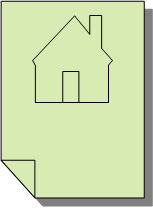
\includegraphics[width=0.25\textwidth]{figures/Homepage-icon.png}
  \end{center}
  \caption{Homepage icon}
  \label{fig:homepageicon}
\end{figure}

\begin{table}[!ht]
  \begin{center}
    \caption{Configurations tested}
    \label{tab:configstested}
    \begin{tabular}{l|c} % <-- Alignments: 1st column left, 2nd middle and 3rd right, with vertical lines in between
      \textbf{Configuration} & \textbf{Description} \\
      \hline
      1 & Simple test with one server\\
      2 & Simple test with one server\\
    \end{tabular}
  \end{center}
\end{table}
% \todo[inline, backgroundcolor=kth-lightblue]{Testade konfigurationer}

\section{Implementation …/Modeling/Simulation/…}
\label{sec:implementationDetails}
% \todo[inline, backgroundcolor=kth-lightblue]{Implementering … / modellering / simulering / …}


\subsection{Some examples of coding}

Listing~\ref{lst:helloWorldInC} shows an example of a simple program written
in C code.

\begin{lstlisting}[language={C}, caption={Hello world in C code}, label=lst:helloWorldInC]
int main() {
printf("hello, world");
return 0;
}
\end{lstlisting}


In contrast, Listing~\ref{lst:programmes} is an example of code in Python to
get a list of all of the programs at KTH.

\lstset{extendedchars=true}
\begin{lstlisting}[language={Python}, caption={Using a python program to
    access the KTH API to get all of the programs at KTH}, label=lst:programmes]
KOPPSbaseUrl = 'https://www.kth.se'

def v1_get_programmes():
    global Verbose_Flag
    #
    # Use the KOPPS API to get the data
    # note that this returns XML
    url = "{0}/api/kopps/v1/programme".format(KOPPSbaseUrl)
    if Verbose_Flag:
        print("url: " + url)
    #
    r = requests.get(url)
    if Verbose_Flag:
        print("result of getting v1 programme: {}".format(r.text))
    #
    if r.status_code == requests.codes.ok:
        return r.text           # simply return the XML
    #
    return None
\end{lstlisting}
